\documentclass[11pt]{scrartcl}
%%
%
% This is a poster template with latex macros and using
% the University of Florida Logo.  For further information
% on making postscript, resizeing, and printing the poster file
% please see web site 
% http://www.phys.ufl.edu/~pjh/posters/poster_howto.html
% 
% N.B. This format is cribbed from one obtained from the University
% of Karlsruhe, so some macro names and parameters are in German
% Here is a short glosary:
% Breite: width
% Hoehe: height
% Spalte: column
% Kasten: box
%
% All style files necessary are part of standard TeTeX distribution
% On the UF unix cluster you should not need to import these files
% specially, as they will be automatically located.  If you
% run on a local PC however, you will need to locate these files.
% At UF try /usr/local/TeTeX...
% 
% P. Hirschfeld 2/11/00
%
% The recommended procedure is to first generate a ``Special Format" size poster
% file, which is relatively easy to manipulate and view.  It can be
% resized later to A0 (900 x 1100 mm) full poster size, or A4 or Letter size
% as desired (see web site).  Note the large format printers currently
% in use at UF's OIR have max width of about 90cm or 3 ft., but the paper
% comes in rolls so the length is variable.  See below the specifications
% for width and height of various formats.  Default in the template is
% ``Special Format",  with 4 columns.
%%
%% 
%% Choose your poster size:
%% For printing you will later RESIZE your poster by a factor
%%        2*sqrt(2) = 2.828    (for A0)
%%        2         = 2.00     (for A1) 
%%  
%% 
\def\breite{400mm}     % Special Format. 
\def\hoehe{400mm}      % Scaled by 2.82 this gives 110cm x 90cm 

%\def\breite{390mm}     % Special Format. 
%\def\hoehe{319.2mm}      % Scaled by 2.82 this gives 110cm x 90cm 
\def\anzspalten{2}
%%
%%\def\breite{420mm}     % A3 LANDSCAPE
%%\def\hoehe{297mm}
%%\def\anzspalten{4}
%%
%% \def\breite{297mm}     % A3 PORTRAIT
%% \def\hoehe{420mm}
%% \def\anzspalten{3}
%%
%% \def\breite{210mm}     % A4 PORTRAIT
%% \def\hoehe{297mm}
%% \def\anzspalten{2}
%%
%%
%% Procedure:
%%   Generate poster.dvi with latex
%%   Check with Ghostview
%%   Make a .ps-file with ``dvips -o poster.ps poster''
%%   Scale it with poster_resize poster.ps S
%%   where S is scale factor
%%     for Special Format->A0 S= 2.828 (= 2^(3/2)))
%%     for Special Format->A1 S= 2 (= 2^(2/2)))
%% 
%% Sizes (European:)
%%   A3: 29.73 X 42.04 cm
%%   A1: 59.5 X 84.1 cm
%%   A0: 84.1 X 118.9 cm
%%   N.B. The recommended procedure is ``Special Format x 2.82"
%%   which gives 90cm x 110cm (not quite A0 dimensions).
%%
%% --------------------------------------------------------------------------
%%
%% Load the necessary packages
%% 
\usepackage{palatino}
\usepackage[latin1]{inputenc}
\usepackage{epsf}
\usepackage{graphicx,psfrag,color,pstcol,pst-grad}
\usepackage{amsmath,amssymb}
\usepackage{latexsym}
\usepackage{calc}
\usepackage{multicol}
%\usepackage[]{graphicx}
\usepackage{epstopdf}
%%
%% Define the required numbers, lengths and boxes 
%%
\newsavebox{\dummybox}
\newsavebox{\spalten}
%\input psfig.sty

%%
%%
\newlength{\bgwidth}\newlength{\bgheight}
\setlength\bgheight{\hoehe} \addtolength\bgheight{-1mm}
\setlength\bgwidth{\breite} \addtolength\bgwidth{-1mm}

\newlength{\kastenwidth}

%% Set paper format
\setlength\paperheight{\hoehe}                                             
\setlength\paperwidth{\breite}
\special{papersize=\breite,\hoehe}

\topmargin -1.0in
\marginparsep0mm
\marginparwidth0mm
\headheight0mm
\headsep0mm


%% Minimal Margins to Make Correct Bounding Box
%\setlength{\oddsidemargin}{-2.44cm}
%\addtolength{\topmargin}{-3mm}
\setlength{\oddsidemargin}{-2.44cm}
\addtolength{\topmargin}{-3mm}
\textwidth\paperwidth
\textheight\paperheight

%%
%%
\parindent0cm
\parskip1.5ex plus0.5ex minus 0.5ex
\pagestyle{empty}




\definecolor{recoilcolor}{rgb}{1,0,0}
\definecolor{occolor}{rgb}{0,1,0}
\definecolor{pink}{rgb}{0,1,1}





\def\UberStil{\normalfont\sffamily\bfseries\large}
\def\UnterStil{\normalfont\sffamily\small}
\def\LabelStil{\normalfont\sffamily\tiny}
\def\LegStil{\normalfont\sffamily\tiny}

%%
%% Define some commands
%%
\definecolor{JG}{rgb}{0.1,0.9,0.3}

\newenvironment{kasten}{
  \begin{lrbox}{\dummybox}
    \begin{minipage}{\linewidth}}
    {\end{minipage}
  \end{lrbox}
  \raisebox{-\depth}{\psshadowbox[cornersize=absolute,linearc=14pt,framesep=1em]{\usebox{\dummybox}}}\\[0.5em]}
\newenvironment{spalte}{
  \setlength\kastenwidth{1.2\textwidth}
  \divide\kastenwidth by \anzspalten
  \begin{minipage}[t]{\kastenwidth}}{\end{minipage}}

%\renewcommand{\emph}[1]{{\color{red}\textbf{#1}}}


%\def\op#1{\hat{#1}}
\begin{document}
%%%%%%%%%%%%%%%%%%%%%%%%%%%%%%%%%%%%%%%%%%%%%%%%%%%%
%%%               Background                     %%%
%%%%%%%%%%%%%%%%%%%%%%%%%%%%%%%%%%%%%%%%%%%%%%%%%%%%
%{\newrgbcolor{gradbegin}{0.5 0.5 1}
%  \newrgbcolor{gradend}{1 1 1}%{1 1 0.5}%
%  %\rput[cm](15.23,-15){
%  \rput[tl]{0}(0,0){
%  %\includegraphics[width=\paperwidth]{logos/antenna1} %lower resolution
%  %\includegraphics[width=\paperwidth]{logos/antenna2} %higher resolution
%  }
%\vfill}

%{\newrgbcolor{gradbegin}{0.5 0.5 1}%
%  \newrgbcolor{gradend}{1 1 1}%{1 1 0.5}%
%  \psframe[fillstyle=gradient,gradend=gradend,%
%  gradbegin=gradbegin,gradmidpoint=0.1](\bgwidth,-\bgheight)}
%\vfill
%%%%%%%%%%%%%%%%%%%%%%%%%%%%%%%%%%%%%%%%%%%%%%%%%%%%
%%%                     Header                   %%%
%%%%%%%%%%%%%%%%%%%%%%%%%%%%%%%%%%%%%%%%%%%%%%%%%%%%
      
\includegraphics[width=40cm,height=5cm]{../img/header_clean}

\hfill
\psshadowbox{\makebox[0.87\textwidth]{%
    \parbox[c]{0.87\linewidth}{%
      \begin{center}
		\textbf{\Huge {ALMA Software Regression Tests: The Evolution under an
Operational Environment}}\\[0.5em]
        \textsc{\large Ruben Soto$^a$, V\'ictor Gonz\'alez$^a$, Jorge Ibsen$^b$, Matias Mora$^a$, Norman S\'aez$^a$, Tzu-Chiang Shen$^a$}\\[0.3em]
        { $^a$Associated Universities, Inc. (AUI), Santiago, Chile;}\\
        { $^b$European Southern Observatory (ESO), Santiago, Chile;}
      \end{center}}
\hfill}}\hfill\mbox{}\\

\hfill
\psshadowbox{\makebox[0.87\textwidth]{%
    \hfill
    \parbox[t]{0.85\linewidth}{%
\hfill{\large\bf{\color{red}ABSTRACT}}\hfill\mbox{}\\
The ALMA software is a large collection of software modules, which implements
the functionality needed for the observatory day-to-day operation. Many
software patches must periodically be applied to fix problems detected during
operations or to introduce enhancements into the system identified after a
release has been deployed. Under this scenery, it has been imperative to
establish, besides a strict configuration control system, a weekly regression
test to ensure that modifications applied do not impact system stability. A
test suite has been developed for this purpose, which reflects the operations
performed by the commissioning and operations groups, and that aims to detect
problems associated to the changes introduced at different versions of ALMA
software releases. This paper presents the evolution of the regression test
suite. Topics about the selection of the tests to be executed, the validation
of the data obtained and the automation of the test suite are also presented.
}
\hfill}}\hfill\mbox{}

\begin{lrbox}{\spalten}
  \parbox[t][0.41\textheight]{1.3\textwidth}{
   % \vspace*{0.2cm}
%%%%%%%%%%%%%%%%%%%%%%%%%%%%%%%%%%%%%%%%%%%%%%%%%%%%
%%%                 first column                 %%%             
%%%%%%%%%%%%%%%%%%%%%%%%%%%%%%%%%%%%%%%%%%%%%%%%%%%%
    \begin{spalte}
     
      \begin{kasten}
		\section*{\hspace{0.1cm} {\color{blue}The tests upgrade and environment standardization}}
%\vspace{0.1cm}
			\begin{minipage}[t]{0.95\linewidth}
\vspace{-0.5cm}
At the beggining, the regression test suite was strongly oriented to new features testing and verification of bug fixes. 
Under an operational environment, those tests were focused on reproducing, as much as possible, the activities that science 
and engineering groups performed on a daily basis. 
Most of these tests derived from python scripts developed by science and engineering groups. Tests oriented to prove the automatic 
mode of the ALMA telescope were also included in the suite. An additional section to validate the data obtained from the 
astronomical observations was added. By the other hand, due to the limited testing time with real hardware, the possibility of 
running the regression tests suite in a simulated environment acquired more importance. A significant effort was done to 
standardize the testing environment in order to reproduce, as much as possible, the operational configuration. The progress 
on the hardware and software development demanded more functionality to be tested, and the regression testing suite was adapted 
to assume the new challenges.\\ 
\begin{center}\includegraphics[width=15cm,height=!]{../img/reg-tests-workflow-2}\end{center}
\begin{center}\textit{Current structure of the Regression Tests Procedure}\end{center}
\end{minipage} \vspace{-0.2cm}

        \section*{\hspace{0.3cm} {\color{blue} Validation of science data}}
            \vspace{-0.5cm}
			\begin{minipage}[l]{0.50\linewidth}
            In normal operations, the data sets are the product of observations that are delivered to the principal 
            investigator, and thus their consistency is vital. Also, the purpose of the whole on-line software chain is to produce 
            these data sets, thus it is normal that validating them became a major target. Although when operating in simulation 
            there are many features that do not produce sensible simulated data, like the one a user would obtain when observing 
            a real astronomical source, the consistency of the generated project can still be validated. The ALMA software supports a complete data analysis toolkit 
            called CASA (Common Astronomy Software Applications), also used for other projects, which provides all necessary tools through python 
            libraries that can be used to produce custom reduction scripts. 
            An improved data validation strategy was implemented. The new approach consists of executing an end-to-end interactive (automatic) observation and then 
            plotting the resulting data set, which can be validated through visual inspection.

			\end{minipage}
            \hspace{0.7cm}
			\begin{minipage}[r]{0.40\linewidth}
            \vspace{-0.3cm}
            \includegraphics[width=9cm,height=!]{../img/casa-reduction}
            \begin{center}\textit{Fringe pattern validation by using CASA off-line tool.}\end{center}
			\end{minipage}
			\vspace{0.08cm}
      \end{kasten}

    \end{spalte}
	 \hfill
%%%%%%%%%%%%%%%%%%%%%%%%%%%%%%%%%%%%%%%%%%%%%%%%%%%%
%%%               second column                  %%%             
%%%%%%%%%%%%%%%%%%%%%%%%%%%%%%%%%%%%%%%%%%%%%%%%%%%%
    \begin{spalte}
       
      \begin{kasten}
        \section*{\hspace{0.1cm} {\color{blue} Automation of regression test suite}}
			\begin{minipage}[t]{0.95\linewidth}
\vspace{-0.3cm}
%\begin{minipage}[l]{0.40\linewidth}
As a consequence of new software functionalities, the test procedures became
more complex and also demanded more time to be executed. Therefore, the need
for introducing some level of automation was imperative to optimize the testing
process. For automation purposes, the pyunit framework fulfilled most
requirements for the execution of the testing tasks. Thus, manual testing
procedures were translated into python scripts and executed as pyunit tasks.

%\end{minipage}
%\hspace{1cm}
%\begin{minipage}[r]{0.50\linewidth}
 \vspace{0.1cm}
\begin{center}\includegraphics[height=9cm]{../img/UMLmodel}\end{center}
\begin{center}\textit{UML diagram of the Automatic Regression Testing framework.}\end{center}
%\end{minipage}
\vspace{-0.5cm}
			\end{minipage} 
\vspace{1cm}

Further, a python framework was implemented to integrate all those tests in a unique suite 
that allowed a coordinated execution with common parameters. This framework was also responsible 
for the system startup and the allocation of resources needed for test executions, without human 
intervention. The adaptability of the tests suite by adding or removing tests in a dynamic and 
efficient way was another point considered as requirement for the implementation of the framework.
In practical terms, the testing framework was composed by python classes and 
packages implemented for every specific purpose
In addition to the improvements at the time required for the test execution, 
the framework also granted a level of flexibility at the definition of the suite by 
depending of the verification scope. Thus, the users are able to select only basic 
tests or part of the astronomical observations (manual or automatic observations) 
in a dynamic way.
      \end{kasten}

    \end{spalte}
	 \hfill\mbox{}

}
\end{lrbox}
\hfill
\resizebox*{0.95\textwidth}{!}{
  \usebox{\spalten}}\hfill\mbox{}

\vspace{1.6cm}
\hspace{1cm}
\psshadowbox[cornersize=absolute,linearc=14pt]{\makebox[0.923\textwidth]{%
	 \hfill
    \parbox[t]{0.9\linewidth}{
\begin{minipage}[t]{0.49\linewidth}
\vspace{0.1cm}
\section*{ {\normalsize \color{red} Conclusions}}

\vspace{-0.2cm}
{\footnotesize
\renewcommand{\baselinestretch}{0.3}
The evolution of the regression test suite has produced considerable benefits
to the overall software testing process.  The automation of the test suite
decreased dramatically the amount of time required to verify a software
release. This improvement allowed the Software Group to make a
more efficient use of time available on the real hardware. 
%set of new functionalities added incrementally to the ALMA software and
%delivered systematically in a short time schedule (~every 2 week), the
%regression test suite played a fundamental role to guarantee software stability
%for the main operations.  and troubleshooting of issues that cannot be
%reproduced in a simulated environment. On the other hand, with the introduction
%of the 
}
\vspace{0.1cm}
\end{minipage}\hfill
\begin{minipage}[t]{0.49\linewidth}
\vspace{0.8cm}
{\footnotesize
\renewcommand{\baselinestretch}{0.5}
Despite there are a lot of pending improvements to the current regression test process, until this point most 
efforts were concentrated on turning the regression test suite into a tool that actively contributes to the 
stabilization of the software development process, by guarantying the functionality required to continue 
with acceptance and commissioning activities of the ALMA Observatory.

%As mentioned above, there are a lot of pending improvements to the current
%procedures. However, until this point most efforts were concentrated on turning
%the regression test suite into a tool that actively contributes to the
%stabilization of the software development process, by guarantying the
%functionality required to continue with acceptance and commissioning activities
%of the ALMA Observatory.
}
\end{minipage}
}
\hfill}}\hfill\mbox{}\\
%\vfill
%\vspace{-0.1cm}

\hfill
\psshadowbox{\makebox[0.9\linewidth]{
\hfill
%\begin{minipage}[t]{0.28\linewidth}
%\vspace{0.1cm}
%{\scriptsize
%{\small\bf Acknowledgements}
%
%\renewcommand{\baselinestretch}{0.5}
%}
%\vspace{0.2cm}
%\end{minipage} \hfill

\begin{minipage}[t]{0.9\linewidth}
\vspace{0.1cm}
{\scriptsize
\renewcommand{\baselinestretch}{1.0}
{\small\bf References}

[1] Lopez, B. and et all, R. A., ``Software regression testing: practical experience at the alma test facility'', in
[{\em Advanced Software and Control for Astronomy II}{\hspace{0.1em}}] Proc. SPIE 7019, 97-97 (2008).
\renewcommand{\baselinestretch}{0.5}

[2] Gonzalez, V., Mora, M., Araya, R., Arredondo, D., Bartsch, M., Burgos, P., Ibsen, J., Reveco, J., Saez, N.,
Schemrl, A., Sepulveda, J., Shen, T., Soto, R., et all., ``First year of alma site software deployment: where everything comes together'',{\hspace{0.1em}} Proc. SPIE 7737 (2010).
\renewcommand{\baselinestretch}{0.5}

[3] Mora, M., Ibsen, J., Kern, J., Araya, R., Troncoso, N., Gonzalez, V., Marson, R., Juerges, T., Farris, A.,
and Reyes, C., ``Hardware device simulation framework in the alma control subsystem'',{\hspace{0.1em}} Proc. ADASS XVIII 411 (2008).
\renewcommand{\baselinestretch}{0.5}

[4] Mora, M., Avarias, J., Tejeda, A., Gil, J., and Sommer, H., ``Alma software scalability experience with
growing number of antennas'', Proc. SPIE 8451-31 (2012).
\renewcommand{\baselinestretch}{0.5}

[5] Petry, D., ``Analysing alma data with casa'', Proc. ADASS XXI (2012). http://arxiv.org/abs/1201.3454.
\renewcommand{\baselinestretch}{0.5}

[6] Shen, T., Ibsen, J., Olguin, R., and et all., R. S., ``Status of alma software'', Proc. ICALEPCS (2011).
\renewcommand{\baselinestretch}{0.5}

}
\hfill
\end{minipage}
}}\hfill\mbox{}

%
%\hfill
%\psshadowbox{\makebox[0.95\linewidth]{
%}}\hfill\mbox{}


%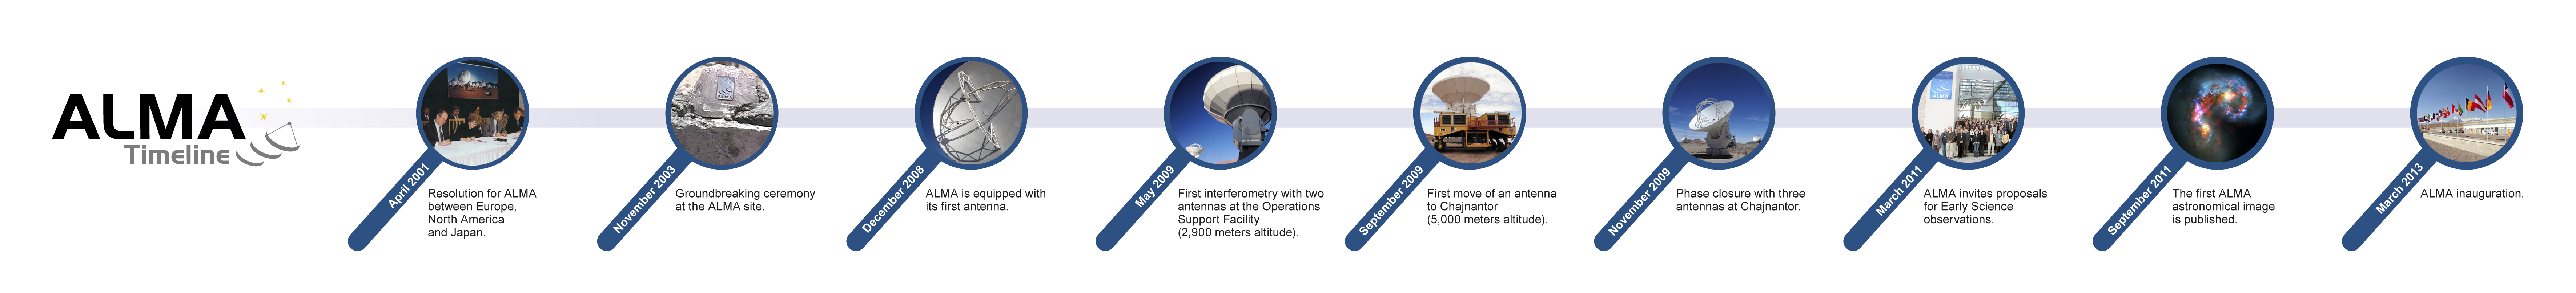
\includegraphics[width=40cm,height=5cm]{../img/footer_timeline}

\includegraphics[width=40cm,height=5cm]{../img/footer_map_text}

\end{document}
